\documentclass[11pt,a4paper]{article}

\usepackage[margin=25mm]{geometry}
\usepackage[T1]{fontenc}
\usepackage[utf8]{inputenc}
\usepackage{lmodern}
\usepackage{microtype}
\usepackage{amsmath,amssymb}
\usepackage{booktabs,tabularx,array}
\usepackage{xcolor}
\usepackage{hyperref}
\usepackage{enumitem}
\usepackage{tikz}
\usetikzlibrary{arrows.meta,positioning,shapes.geometric}

\definecolor{BloomSage}{HTML}{4A7C59}
\definecolor{BloomInk}{HTML}{26352C}
\definecolor{BloomPale}{HTML}{E7F0E7}
\hypersetup{
  colorlinks=true,
  linkcolor=BloomSage,
  urlcolor=BloomSage,
  pdftitle={Bloom: Facial Skin Image Analysis with Classical DIP},
  pdfauthor={Bloom Project Team}
}
\setlist{itemsep=3pt,topsep=4pt}
\renewcommand{\arraystretch}{1.2}

\title{\textbf{Bloom: Facial Skin Image Analysis}\[3pt]
\large A Digital Image Processing Project Overview}
\author{DIP Course Project \\ Rajiv Gandhi Institute of Petroleum Technology}
\date{\today}

\begin{document}
\maketitle

\begin{abstract}
Bloom is an educational web application that demonstrates a classical digital image processing (DIP) pipeline on facial photographs. It validates an image, locates a face and candidate skin area, enhances luminance, computes spatial- and frequency-domain responses, and visualizes relative colour and texture patterns. The application is designed to make intermediate processing stages inspectable. Its outputs are image-based estimates: they are not diagnoses, clinically validated severity scores, or measured detection accuracy.
\end{abstract}

\tableofcontents
\newpage

\section{Project at a glance}

\subsection{Problem addressed}
Skin photographs vary with illumination, focus, camera processing, pose, and background. A raw image is therefore a difficult input for a simple pixel threshold, while an opaque final score does not help a student explain what an algorithm actually did. Bloom addresses this educational and visualization problem by applying a sequence of standard image-processing operations and displaying intermediate images beside the final relative measurements.

The project does \emph{not} solve the clinical problem of diagnosing acne, pigmentation, or other skin conditions. Classical image operations can locate colour or frequency patterns, but cannot establish that a pattern is a disease.

\subsection{Project objectives}
\begin{itemize}
  \item Demonstrate practical DIP operations on a facial image: colour-space conversion, enhancement, segmentation, filtering, thresholding, morphology, connected components, and visualization.
  \item Constrain measurements to a face-derived region rather than thresholding the entire photograph.
  \item Show how intermediate signals change through the pipeline, including low-pass, high-pass, Difference of Gaussians (DoG), and FFT band-pass views.
  \item Report relative image measurements with explicit limitations and without claiming unverified accuracy.
\end{itemize}

\subsection{Intended use and output}
The user uploads a JPEG or PNG image (maximum 5 MB). Bloom returns an original and enhanced view, skin-region visualization, frequency-response views, concern overlays, an appearance index, and processing-stage timings. Images are processed in memory; the account history stores scan measurements rather than the source image.

\section{System architecture}

The browser sends an image to a FastAPI endpoint. The backend validates the upload and runs the image pipeline. It serializes the image views and measurements as a JSON response. The React interface presents the result and the processing grid. The optional routine module is a separate rule-based feature and is not part of the DIP measurement pipeline.

\begin{figure}[ht]
\centering
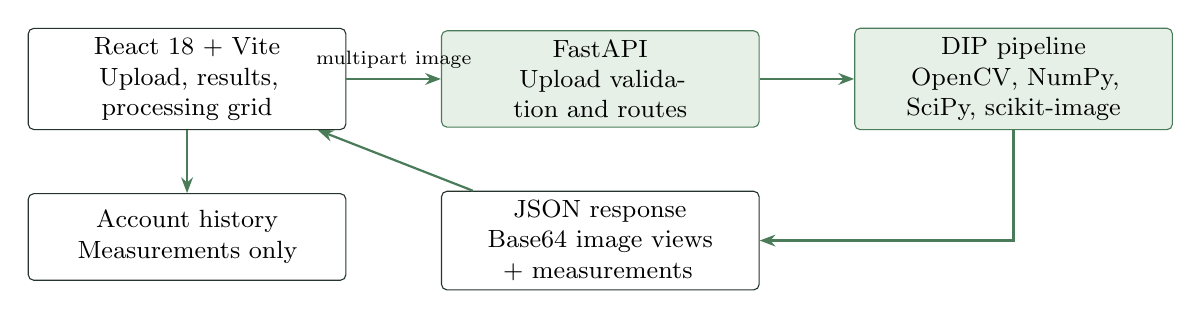
\begin{tikzpicture}[
  node distance=8mm and 12mm,
  block/.style={draw=BloomSage, fill=BloomPale, rounded corners=2pt,
    align=center, text width=38mm, minimum height=11mm, font=\small},
  io/.style={draw=BloomInk, fill=white, rounded corners=2pt,
    align=center, text width=38mm, minimum height=11mm, font=\small},
  arrow/.style={-{Stealth[length=2mm]}, thick, draw=BloomSage}
]
\node[io] (browser) {React 18 + Vite\\Upload, results, processing grid};
\node[block, right=of browser] (api) {FastAPI\\Upload validation and routes};
\node[block, right=of api] (pipeline) {DIP pipeline\\OpenCV, NumPy, SciPy, scikit-image};
\node[io, below=of api] (response) {JSON response\\Base64 image views + measurements};
\node[io, below=of browser] (history) {Account history\\Measurements only};
\draw[arrow] (browser) -- node[above,font=\scriptsize]{multipart image} (api);
\draw[arrow] (api) -- (pipeline);
\draw[arrow] (pipeline) |- (response);
\draw[arrow] (response) -- (browser);
\draw[arrow] (browser) -- (history);
\end{tikzpicture}
\caption{High-level application architecture. The default scan uses the classical DIP path; MediaPipe supplies pretrained face landmarks.}
\label{fig:architecture}
\end{figure}

\subsection{Main software components}
\begin{tabularx}{\textwidth}{@{}p{0.27\textwidth}X@{}}
\toprule
\textbf{Component} & \textbf{Role} \\
\midrule
\texttt{frontend/} & React interface for sign-in, photo selection, analysis results, and the stage-by-stage processing grid. \\
\texttt{backend/main.py} & FastAPI routes, file checks, API response formatting, and optional account/history operations. \\
\texttt{backend/pipeline.py} & Orchestrates preprocessing, enhancement, segmentation, frequency decomposition, masks, post-processing, and visualization. \\
\texttt{backend/src/} & Focused DIP modules for enhancement, segmentation, frequency operations, thresholding, post-processing, and image output. \\
\texttt{backend/routine.py} & Separate rule-based routine feature. It is not an image-processing or diagnostic model. \\
\texttt{start.ps1} & Starts the local FastAPI backend and Vite development server. \\
\bottomrule
\end{tabularx}

\section{How one image is processed}

The backend resizes the decoded RGB image to $512\times512$ before the core stages. A quality gate checks mean grayscale brightness and Laplacian variance. A face landmark pass then constrains the candidate skin mask. If the quality gate or face detection fails, analysis returns an error rather than measuring arbitrary background pixels.

\begin{enumerate}
  \item \textbf{Input checks:} accept supported image content, decode, resize, and check exposure and focus.
  \item \textbf{Enhancement:} shift mean LAB luminance, apply CLAHE on the luminance channel, then bilateral smoothing.
  \item \textbf{Face and skin region:} obtain MediaPipe FaceMesh landmarks; create a face oval; combine YCrCb and HSV ranges for candidate skin; clean the mask and exclude eyes, brows, lips, and nose.
  \item \textbf{Feature responses:} compute low-pass, high-pass, DoG, and LAB channels from the enhanced image.
  \item \textbf{Candidate masks:} threshold relative redness, darkness, and DoG response inside the analysis region.
  \item \textbf{Cleanup and regions:} apply morphology, remove small connected components, and calculate area, region count, centroid, and bounding box.
  \item \textbf{Independent FFT view:} calculate a radial Gaussian band-pass response, threshold its magnitude inside the skin region, then clean and outline the selected regions.
  \item \textbf{Presentation:} encode original, enhanced, masks, frequency maps, and overlays; return those with relative measurements and timings.
\end{enumerate}

\section{DIP concepts: where, how, and why}

\small
\begin{tabularx}{\textwidth}{@{}p{0.17\textwidth}p{0.23\textwidth}X p{0.2\textwidth}@{}}
\toprule
\textbf{Concept} & \textbf{Where used} & \textbf{How it is used} & \textbf{Purpose and caveat} \\
\midrule
Brightness and focus checks & \texttt{preprocessing.py} & Mean grayscale value and variance of the Laplacian are compared with fixed limits. & Reject very dark, overexposed, or blurred inputs. Limits are prototype values, not calibrated camera-independent quality standards. \\
LAB luminance shift & \texttt{enhancement.py} & The mean of the L channel is shifted toward 130, with values clipped to 8-bit range. & Global brightness normalization. It does not correct spatially varying illumination. \\
CLAHE & \texttt{enhancement.py} & CLAHE is applied to LAB L with clip limit 2 and an $8\times8$ tile grid. & Improve local luminance contrast without separately equalizing RGB channels. It may also amplify noise or fine skin texture. \\
Bilateral filter & \texttt{enhancement.py} & OpenCV bilateral filtering follows CLAHE using $d=9$, $\sigma_{color}=75$, and $\sigma_{space}=75$. & Smooth nearby colours while preserving some edges; strong smoothing can still alter fine texture. \\
Face-constrained segmentation & \texttt{skin\_segmentation.py} & FaceMesh supplies an oval; YCrCb and HSV threshold masks are intersected, morphologically cleaned, and facial features excluded. & Restrict analysis to a candidate facial skin region. Fixed colour ranges remain sensitive to lighting, makeup, and skin appearance. \\
Gaussian low/high-pass & \texttt{frequency\_decomposition.py} & A $(21,21)$ Gaussian low-pass is subtracted from grayscale intensity to produce a centred high-pass view. & Separate broad shading from fine intensity changes. The displayed high-pass contrast is adjusted for visibility. \\
Difference of Gaussians & \texttt{frequency\_decomposition.py}, \texttt{lesion\_detection.py} & Compute $G_{\sigma=1}*I-G_{\sigma=3}*I$; threshold the absolute response relative to the ROI maximum. & Illustrate a spatial band-pass/blob-like response. It does not identify acne; a maximum-based threshold is vulnerable to outliers. \\
LAB opponent channels & \texttt{lesion\_detection.py} & Compare LAB A values above ROI mean and L values below ROI mean, each with a standard-deviation multiplier and minimum offset. & Produce relative red-contrast and dark-region masks. These are image contrasts, not biological redness or confirmed pigmentation. \\
Adaptive statistical threshold & \texttt{thresholding.py} & Use $\mu+\max(\delta,k\sigma)$ for high-valued foreground or $\mu-\max(\delta,k\sigma)$ for low-valued foreground, with statistics from ROI pixels. & Adapt threshold to the image ROI while protecting pixels outside it. Parameters remain hand-set and unvalidated. \\
Distance transform and watershed & \texttt{lesion\_detection.py} & Distance transform peaks become markers; watershed on negative distance separates touching candidate regions. & A standard component-splitting heuristic. Marker placement can split or merge incorrectly; region counts are not validated lesion counts. \\
Morphology and connected components & \texttt{postprocessing.py} & A small opening removes speckles; 8-connected components below 50 pixels are dropped; region properties and relative area are measured. & Clean masks and describe their geometry. The 50-pixel cutoff depends on resizing and is not biologically calibrated. \\
2D FFT Gaussian band-pass & \texttt{frequency\_domain.py}, \texttt{imperfection\_map.py} & Radial frequency cutoffs 0.02 and 0.25 of the minimum image dimension define a band-pass. Absolute response is thresholded at ROI mean plus 1.5 standard deviations. & Visualize relative mid-frequency detail. No physical lesion scale or annotated calibration supports the cutoffs; the output is not a disease detector. \\
ITA appearance index & \texttt{skin\_tone.py} & Convert 8-bit OpenCV LAB to $L^*$ and $b^*$, calculate per-pixel $\arctan((L^*-50)/b^*)$, then report the median angle and a named appearance band. & A colour descriptor from the image ROI, affected by illumination and camera colour processing. It is not skin type, race, ethnicity, or a clinical category. \\
\bottomrule
\end{tabularx}
\normalsize

\section{What is distinctive about Bloom?}

\begin{itemize}
  \item \textbf{Inspectable processing:} the results grid shows the actual input, enhancement, skin mask, low/high-pass images, DoG response, FFT heatmap, selected surface regions, and final overlay. It supports a DIP explanation rather than presenting only one opaque number.
  \item \textbf{A classical image-processing core:} the default analysis does not require a custom-trained skin-disease classifier or a GPU. MediaPipe FaceMesh is a pretrained landmark component; the colour, frequency, threshold, and morphology measurements are classical CV.
  \item \textbf{Multiple domains shown together:} the project demonstrates spatial filtering, colour-space analysis, morphology, region properties, and Fourier-domain filtering in one user flow.
  \item \textbf{Honest output framing:} the API returns relative extents and prototype variation labels and does not claim measured accuracy on unlabelled uploads.
  \item \textbf{End-to-end implementation:} the project links a web UI, an API, in-memory image handling, a modular pipeline, and explanatory visual output.
\end{itemize}

These are educational and engineering strengths, not evidence that the masks are accurate or clinically useful.

\section{What Bloom currently measures}

The project returns three threshold-based concern maps: surface-anomaly-like DoG candidates, relative redness contrast, and dark-region contrast. It also returns an FFT surface-detail heatmap and selected-region overlay, a median ITA appearance descriptor, and area/count measurements for cleaned masks. Severity-style values in the API are prototype variation bands based on fixed area thresholds. They are not clinical severity grades or confidence scores.

\section{Limitations and evaluation status}

\begin{itemize}
  \item No independent annotated ground-truth set currently establishes precision, recall, F1, IoU, or clinical accuracy.
  \item Fixed thresholds are not calibrated across cameras, lighting setups, makeup, pose, image compression, or skin appearance.
  \item A face landmark model identifies a face geometry; the intersected colour mask is still only a candidate skin segmentation.
  \item DoG maxima, FFT band energy, LAB contrast, and connected-component area can respond to noise, hair, shadows, highlights, pores, or compression artifacts.
  \item Resizing all input images to $512\times512$ makes computation convenient but does not make physical feature scales equivalent across source photographs.
  \item The displayed processing grid appears after the request completes; it visualizes returned intermediate images rather than streaming each backend stage live.
  \item The optional routine engine is a separate rule-based prototype and should not be presented as treatment advice derived from an image.
\end{itemize}

For a defensible evaluation, annotate masks independently, split by subject or source image, compare thresholds on a development set, and report precision, recall, F1, and IoU on an untouched test set. Show failures and sample counts. Do not report an accuracy number from unlabeled uploads.

\section{Presentation summary}

\begin{quote}
Bloom is an educational facial image-analysis application that demonstrates a classical DIP pipeline. It combines luminance enhancement, face-constrained skin masking, LAB colour contrast, Gaussian and DoG filtering, ROI-adaptive thresholding, watershed, morphology, connected components, and a separate FFT band-pass visualization. Its contribution is an inspectable end-to-end demonstration of these operations; its outputs are relative visual estimates, and detection accuracy has not been established with independent ground truth.
\end{quote}

\end{document}
